\chapter{Composici\'{o}n de se\~{n}ales}

\section{Composici\'{o}n de se\~{n}ales}

Mediante la aplicaci\'{o}n de diferentes operaciones matem\'{a}ticas a
dos o m\'{a}s se\~{n}ales se pueden generar o componer nuevas se\~{n}ales.

\subsection{Ventanas rectangulares}

\begin{enumerate}
	\item Consideremos las siguientes se\~{n}ales generadas mediante
	diferencias de escalones unitarios
	\begin{eqnarray}
		x_{c}(t)        &=&     u(t) - u(t-2),                          \label{pulsocont}\\
		x_{d}[n]        &=&     u[n] - u[n-2].                          \label{pulsodisc}
	\end{eqnarray}
	Vea las figuras (\ref{compescconteps.1}) y (\ref{compescdisceps}).
	Este tipo de se\~{n}ales, al multiplicar a otra se\~{n}al, nos permite
	extraer determinados intervalos en el dominio del tiempo. Esta
	operaci\'{o}n se denomina ``windowing'' o aventanamiento.
	
	\item Las se\'{n}ales definidas en (\ref{pulsocont}) y
	(\ref{pulsodisc}) act\'{u}an como selectoras o ventanas
	\begin{eqnarray}
		x_{1}( t)       &=& t x_{c}(t),                                \\
		x_{2}( t)       &=& (t - 2) x_{c}(t - 2),                      \\
		x_{3}( t)       &=& t x_{c}(t) - (t - 2) x_{c}(t - 2),          \\
		x_{4}[ n]       &=& n^{2} x_{d}[n],                             \\
		x_{5}[ n]       &=& n x_{d}[n-4],                               \\ 
		x_{6}[ n]       &=& n^{2} x_{d}[n] - n x_{d}[n-4].
	\end{eqnarray}
	Vea las figuras (\ref{compcontunoeps}) y (\ref{compcontdoseps}). 
\end{enumerate}

\subsection{Sumatoria de se\~{n}ales  desplazadas en el tiempo}

Desplazando en el tiempo ventanas rectangulares y
multiplicandolas por coeficientes adecuados, 
se pueden obtener por sumatoria se\~{n}ales peri\'{o}dicas como la $x_{3}(t)$
\begin{equation}
	x_{3}(t) = \sum_{k=-\infty}^{\infty}  (-1)^k x_{c}(t- T k),
\end{equation}
(Vea la figura (\ref{comppregunoeps})) y la $x_{4}(t)$
\begin{equation}
	x_{4}(t) = \sum_{k=-\infty}^{\infty}  (-1)^k x_{d}[n- N k], 
\end{equation}
(Vea la figura (\ref{comppregdoseps})).

\subsection{Sumatoria de impulsos  desplazadas en el tiempo}

Desplazando en el tiempo impulsos y
multiplicandolas por coeficientes adecuados, 
se pueden obtener por sumatoria se\~{n}ales peri\'{o}dicas como la $x_{5}(t)$
\begin{equation}
	x_{5}(t) = \sum_{k=-\infty}^{\infty}  (-1)^k \delta(t- T k),
\end{equation}
y la $x_{6}(t)$
\begin{equation}
	x_{6}(t) = \sum_{k=-\infty}^{\infty}  (-1)^k \delta[n- N k]. 
\end{equation}

\begin{figure}
	\centering
	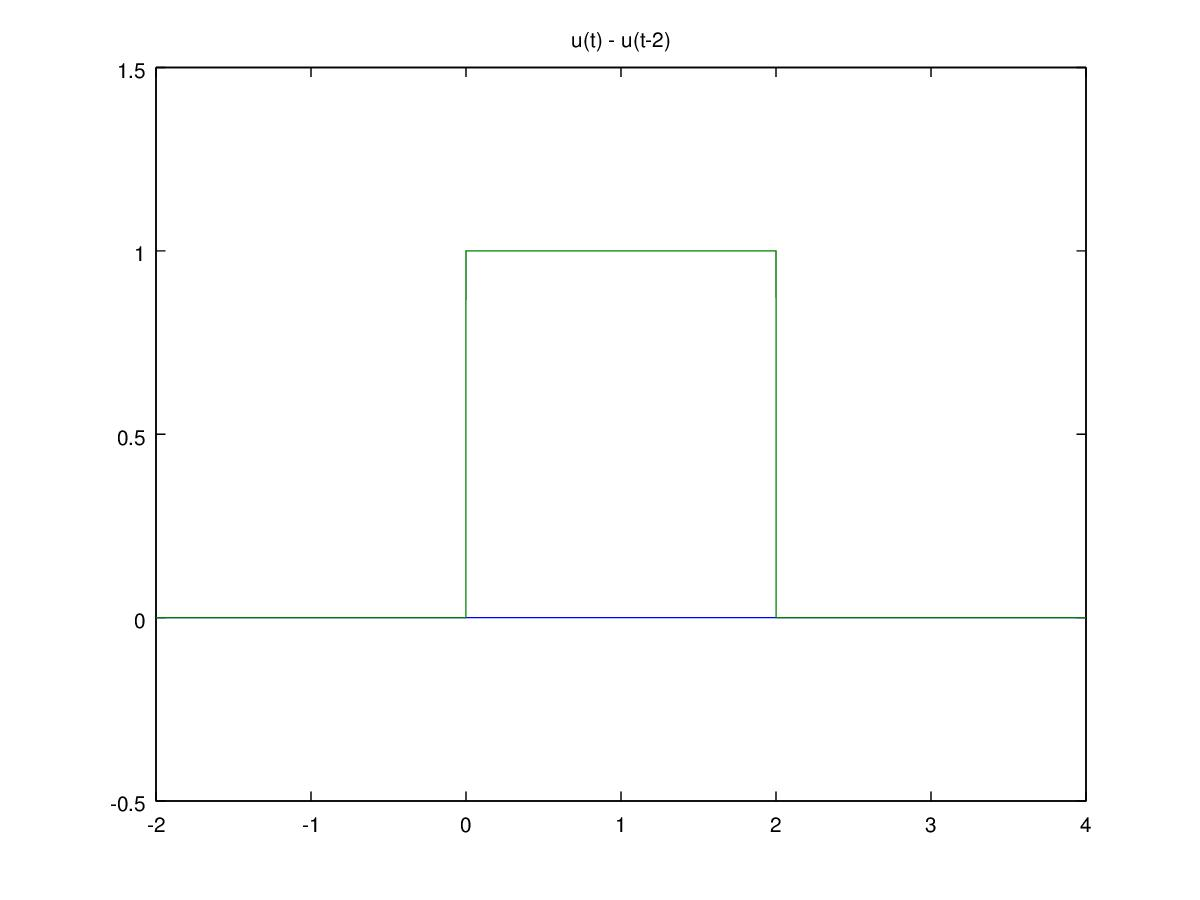
\includegraphics[height=3in]{./graphics/compesccont.eps}
	\caption{Composici\'{o}n de dos escalones para formar una se\~{n}al
		tipo pulso (tiempo continuo)}
	\label{compescconteps.1}
\end{figure}

\begin{figure}
	\centering
	
\includegraphics[height=3in]{./graphics/compcontuno.eps}
	\caption{Composici\'{o}n de se\~{n}ales (tiempo continuo)}
	\label{compcontunoeps}
\end{figure}

\begin{figure}
	\centering
	
\includegraphics[height=3in]{./graphics/compescdisc.eps}
	\caption{Composici\'{o}n de dos escalones para formar un par de
		impulsos (tiempo discreto)}
	\label{compescdisceps}
\end{figure}

\begin{figure}
	\centering
	
\includegraphics[height=3in]{./graphics/compcontdos.eps}
	\caption{Composici\'{o}n de se\~{n}ales (tiempo discreto)}
	\label{compcontdoseps}
\end{figure}

\begin{figure}
	\centering
	
\includegraphics[height=3in]{./graphics/comppreguno.eps}
	\caption{Pregunta sobre composici\'{o}n de se\~{n}ales (tiempo
		continuo)}
	\label{comppregunoeps}
\end{figure}

\begin{figure}
	\centering
	
\includegraphics[height=3in]{./graphics/comppregdos.eps}
	\caption{Pregunta sobre composici\'{o}n de se\~{n}ales (tiempo
		discreto)}
	\label{comppregdoseps}
\end{figure}

\section{Se\~{n}ales de tiempo discreto}

\subsection{El impulso unitario}

Hemos visto que el impulso unitario de tiempo discreto se define como 
\begin{equation}
        \delta \left[ n\right] =\left\{ 
\begin{array}{ll}
0, & n\neq 0, \\ 
1, & n=0.
\end{array}
\right.
\end{equation}

Vea la Fig. (\ref{epsimpunidisc}).

\begin{figure}
        \centering
        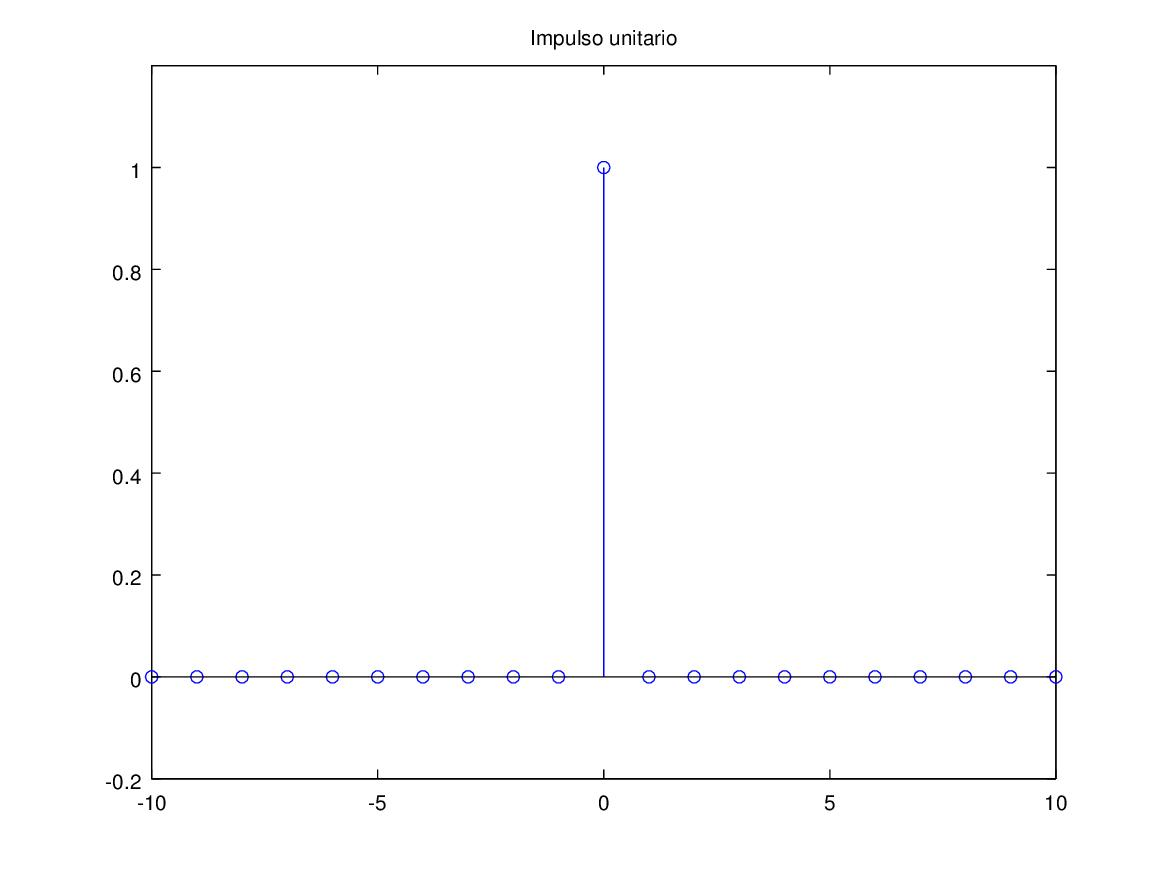
\includegraphics[height=2in]{./graphics/impunidisc.eps}
        \caption{Impulso unitario de tiempo discreto.}
        \label{epsimpunidisc}
\end{figure}

\subsection{El impulso unitario desplazado}

Desplazar un impulso unitario en el tiempo es sencillo. Veamos la
definci\'{o}n de $\delta[n-m]$ (La diferencia con la definici\'{o}n de
$\delta[n]$ aparece resaltada)
\begin{equation}
\delta[n\mathbf{-m}] = \left\{ \begin{array}{cc}
      1 & n  \mathbf{-m} = 0\\
      0 & n  \mathbf{-m} \neq 0 \end{array} 
  \right. \rightarrow
\delta[n\mathbf{-m}] = \left\{ \begin{array}{cc}
      1 & n  = \mathbf{m}\\
      0 & n  \neq \mathbf{m} \end{array} 
  \right.
\end{equation}

\subsection{El impulso multiplicado por un coeficiente}

La multiplicaci\'{o}n de un impulso unitario $\delta[n]$ por un
coeficiente $a$ se define como
\begin{equation}
a \, \delta[n] = \left\{ \begin{array}{cc}
      a & n = 0\\
      0 & n \neq 0 \end{array} 
  \right.
\end{equation}

\subsection{La suma de dos impulsos desplazados en el tiempo y
  multiplicados por coeficientes}

La suma de dos impulsos desplazados en el tiempo y multiplicados por
coeficientes es una combinaci\'{o}n lineal de impulsos. La podemos
definir de la siguiente forma
\begin{equation}
a_{1} \, \delta[n - m_{1}] + 
a_{2} \, \delta[n - m_{2}] = \left\{ \begin{array}{cc}
      a_{1} & n = m_{1}\\
      a_{2} & n = m_{2}\\
      0 & (n \neq m_{1}) \wedge (n \neq m_{2})  \end{array} 
  \right.
\end{equation}


\subsection{La suma de $N$ impulsos desplazados en el tiempos y
  multiplicados por coeficientes}

Podemos definir la suma de $N$ impulsos desplazados en el tiempo y multiplicados por
coeficientes $a_{k}$
\begin{equation}
x[n] = \sum_{k = 1}^{N} a_{k} \, \delta[n - k],
\end{equation}
donde para $m \in N$
\begin{equation}
x[m] = \sum_{k = 1}^{N} a_{k} \, \delta[m - k] = a_{m},
\end{equation}
porque solo donde $m = k$ se cumple $\delta[m - k] = \delta[0] = 1$ y por lo tanto hay un solo impulso igual a $1$ que multiplica al coeficiente $a_{m}$. Todos los otros coeficientes están multiplicados por $0$.

\subsection{La se\~ {n}al como combinaci\'{o}n lineal de impulsos}

\begin{enumerate}

\item Consideremos una sucesi\'{o}n de impulsos 
 $\delta\left[n - n_{0}\right]$, 
(ver Fig.(\ref{convoneeps}) y la Ec. (\ref{claveuno})), multiplicados por los
  respectivos coeficientes  $x\left[n_{0}\right]$, 
  \begin{eqnarray}
    x[-2]\delta \left[ n+2\right]   &=&     \left\{ \begin{array}{ll}
        x[-2],  & n=-2,                 \\ 
        0,      & n\neq -2,
      \end{array}
    \right.                                         \\
    x[-1]\delta \left[ n+1\right]   &=&     \left\{ \begin{array}{ll}
        x[-1],  & n=-1,                 \\ 
        0,      & n\neq -1,
      \end{array}
    \right.                                                 \\
    x[0]\delta \left[ n\right]      &=&     \left\{ \begin{array}{ll}
        x[0],   & n=0,                  \\ 
        0,      & n\neq 0,
      \end{array}
    \right.                                                 \\
    x[1]\delta \left[ n-1\right]    &=&     \left\{ \begin{array}{ll}
        x[1],   & n=1,                  \\ 
        0,      & n\neq 1,
      \end{array}
    \right.                                                 \\
    x[2]\delta \left[ n-2\right]   &=&     \left\{ \begin{array}{ll}
        x[2],   & n=2,                  \\ 
        0,      & n\neq 2,
      \end{array}
    \right.
  \end{eqnarray}
  y en general,
  \begin{equation}
    x[k]\delta \left[ n-k\right] =  \left\{ \begin{array}{ll}
        x[k],   & n=k,          \\ 
        0,      & n\neq k.
      \end{array}
    \right.
  \end{equation}

\item Como podemos ver en la Fig.(\ref{convoneeps}), la suma de
  impulsos desplazados en el tiempo multiplicados por coeficientes
  adecuados equivalen a cualquier se\~{n}al arbitraria $x[n]$.
  \begin{figure}
    \centering
    \includegraphics[width=3in]{./graphics/convone.eps}
    \caption{Una se\~{n}al como suma de impulsos desplazados en el
      tiempo multiplicados por coeficientes adecuados. Los impulsos
      desplazados $\delta[n-k]$ se representan $d[n-k]$.  S\'{o}lo se
      muestran tres impulsos por razones de espacio.}
    \label{convoneeps}
  \end{figure}
        
\item En efecto, agregando m\'{a}s impulsos desplazados y
  multiplicados adecuadamente podemos obtener una expresi\'{o}n que se
  puede escribir en forma general
  \begin{equation}
    x\left[ n\right] =
    \sum_{k=-\infty }^{\infty }x\left[ k\right] \delta \left[n-k\right] .  \label{cduna}
  \end{equation}

\item La Ec. (\ref{cduna}) corresponde a la representaci\'{o}n de una
  secuencia arbitraria $x[n]$ como
  \begin{itemize}
  \item una combinaci\'{o}n lineal de impulsos desplazados $\delta
    \left[ n-k\right]$,
                        
  \item donde los coeficientes de la combinaci\'{o}n lineal son los
    valores $x[k]$.
  \end{itemize}
                
\item Cada impulso desplazado $\delta \left[ n-k\right] $ act\'{u}a
  como selector: suponga que elegimos un valor $n=n_{0}$ y entonces
  tenemos que
  \begin{equation}
    x\left[ n_{0}\right] =
    \sum_{k=-\infty }^{\infty }x\left[ k\right] \delta \left[ n_{0}-k\right] .  
    \label{cddos}
  \end{equation}
                
\item Recordemos la definici\'{o}n de impulso
  \begin{equation}
    \delta \left[ n\right] =\left\{ 
      \begin{array}{cc}
        1, & n=0, \\ 
        0, & n\neq 0.
      \end{array}
    \right.
  \end{equation}
  El impulso ``vale'' $1$ cuando el \'{\i}ndice $n$ (lo que aparece
  entre corchetes) vale $0$. Note que en la ec. (\ref{cddos}) s\'{o}lo
  uno de los infinitos impulsos tiene un \'{\i}ndice nulo,
  espec\'{\i}ficamente
  \begin{equation}
    n_{0}-k=0.
  \end{equation}
  Entonces, de todos los infinitos t\'{e}rminos s\'{o}lo uno es no
  nulo ($k=n_{0})$.  As\'{\i} obtenemos la igualdad
  \begin{equation}
    x\left[ n_{0}\right] =x\left[ n_{0}\right] .
  \end{equation}

\item La utilidad de la ecuaci\'{o}n (\ref{cduna}) es que expresa una
  secuencia
  \begin{equation}
    ...x[-3],x[-2],x[-1],x[0],x[1],x[2],x[3]...
  \end{equation}
  como una sumatoria.

\end{enumerate}

\subsection{La se\~{n}al multiplicada con un impulso}

\begin{enumerate}
\item Consideremos una se\~{n}al $x\left[ n\right]$ a la que
  multiplicamos por un impulso $\delta\left[ n - n_{0}\right]$. 
Hemos probado que
\begin{equation}
x\left[ n\right] \, \delta\left[ n - n_{0}\right] = 
x\left[ n_{0}\right] \, \delta\left[ n - n_{0}\right].
\end{equation}

\item Recordemos que el impulso desplazado $\delta\left[ n - n_{0}\right]$
  act\'{u}a como ``selector'' al multiplicar a una se\~{n}al $x[n]$:
  la \'{u}nica muestra de $x[n]$ multiplicada por $1$ es $x[n_{0}]$,
  todas las dem\'{a}s se multiplican por $0$.

\end{enumerate}

\subsection{Escalado temporal}

\begin{enumerate}
\item Supongamos que tenemos una se\~{n}al $x[n]$ y la usamos para
generar otra se\~{n}al 
\begin{equation}
y[n] = x[3 \, n]. \label{escaladotemporaluno}
\end{equation}
\textquestiondown Qu\'{e} significa la
  Ec. (\ref{escaladotemporaluno})?
Analizemos la siguiente tabla, 

\begin{tabular}{ccc}
$n$ & $x[n]$ & $y[n] = x[3 \, n]$? \\
0   &  $x[0]$ & $x[0]$ \\
& & \\
1   &  $x[1]$ & $x[3]$ \\
& & \\
2   &  $x[2]$ & $x[6]$ \\
& & \\
3   &  $x[3]$ & $x[9]$ \\
& & \\
4   &  $x[4]$ & $x[12]$ \\
& & \\
5   &  $x[5]$ & $x[15]$ \\
& & \\
6   &  $x[6]$ & $x[18]$ \\
... &  ... & ...
\end{tabular}

\item Supongamos que tenemos una se\~{n}al $x[n]$ y la usamos para
generar otra se\~{n}al 
\begin{equation}
y[n] = x[\frac{1}{3} \, n]. \label{escaladotemporaldos}
\end{equation}
\textquestiondown Qu\'{e} significa la Ec. (\ref{escaladotemporaldos})?
Analizemos la siguiente tabla

\begin{tabular}{ccc}
$n$ & $x[n]$  & $x[\frac{n}{3}]$ \\
& & \\
0   &  $x[0]$ & $x[\frac{0}{3}]$ \\
& & \\
1   &  $x[1]$ & $x[\frac{1}{3}]$ ?\\
& & \\
2   &  $x[2]$ & $x[\frac{2}{3}]$ ?\\
& & \\
3   &  $x[3]$ & $x[\frac{3}{3}]$ \\
& & \\
4   &  $x[4]$ & $x[\frac{4}{3}]$ ?\\
& & \\
5   &  $x[5]$ & $x[\frac{5}{3}]$ ?\\
& & \\
6   &  $x[6]$ & $x[\frac{6}{3}]$ \\
& & \\
7   &  $x[7]$ & $x[\frac{7}{3}]$ ?\\
... &  ... & ...
\end{tabular}

Como podemos ver, el problema es que el \'{\i}ndice de una se\~{n}al
de tiempo discreto debe ser un n\'{u}mero entero. Por lo tanto,
deber\'{\i}amos emplear la siguiente definici\'{o}n
\begin{equation}
y[n] = \left\{ \begin{array}{cc}
    x[\frac{n}{3}],      & n = 3 \, m \\
    0,         & n = 3 \, m + 1\\
    0,         & n = 3 \, m + 2
\end{array} \right.
\end{equation}
$\forall m \in N$.

\end{enumerate}

\subsection{Tiempo inverso}

El caso de escalado temporal m\'{a}s sencillo es el del ``viaje al
pasado''. En este caso $y[n] = x[-n]$. Es algo como reproducir un audio "al revés".

Esta es una operación usada en dos casos. Existe un dispositivo denominado scrambler que se puede aplicar a un teléfono: divide el audio en segmentos y después los invierte en tiempo, segmento por segmento, antes de enviarlos por el canal de comunicación. En el otro lado del canal, un dispositivo similar recupera la señal original con el mismo proceso. La idea es que "nadie" pueda espiar la conversación, o mejor dicho que nadie la espíe fácilmente.
También hubo rumores que si se reproducen en tiempo inverso las canciones de rock se pueden oir mensajes ocultos.

Un ejemplo con matlab
\begin{verbatim}
	n = 1:5;
	x = randn(1, 5);
	subplot(2,1,1); stem(n, x); 
	subplot(2,1,2); stem(-n, x);
\end{verbatim}

\subsection{Desplazamiento en el tiempo}

\begin{enumerate}
\item Supongamos una se\~{n}al $x[n]$. Podemos desplazarla en el tiempo
haciendo $y[n] = x[n - n_{0}]$.

\item Por ejemplo, si $x_{1}[n] = cos(2 \, \pi \, \frac{2}{5} \, n)$,
  podemos obtener su versi\'{o}n desplazada cuatro muestras como
  $y_{1} = x_{1}[n - 4] =  cos(2 \, \pi \, \frac{2}{5} \, (n - 4))$.
\end{enumerate}

\subsection{Tren de impulsos}

\begin{enumerate}
\item El impulso unitario est\'{a} definido como
\begin{equation}
\delta[n] = \left\{ \begin{array}{cc}
1 & n = 0, \\
0 & n \neq 0.
\end{array}
\right.
\end{equation}

\item Podemos desplazar el impulso unitario definiendo
\begin{equation}
\delta[n - n_{0}] = \left\{ \begin{array}{cc}
1 & n = n_{0},  \\
0 & n \neq n_{0}.
\end{array}
\right.
\end{equation}

\item Por lo tanto, la siguiente definici\'{o}n 
\begin{equation}
\delta[n - k \, n_{0}] = \left\{ \begin{array}{cc}
1 & n = k \, n_{0},  \\
0 & n \neq k \, n_{0}.
\end{array}
\right.
\end{equation}
donde $k$ es un n\'{u}mero entero, 
nos da impulsos ubicados en m\'{u}ltiplos enteros de $n_{0}$.

\item Si sumamos todos los impulsos obtenidos en el punto anterior,
  obtenemos el tren de impulsos
\begin{equation}
x[n] = \sum_{k=-\infty}^{\infty} \delta[n - k \, n_{0}].
\end{equation}

\end{enumerate}


\section{Se\~{n}ales de tiempo continuo}

\subsection{El pulso}

Un pulso unitario de tiempo continuo $p(t)$ de duraci\'{o}n $\tau$ se define
como una diferencia de escalones unitarios con un factor $\frac{1}{\tau}$
\begin{equation}
  p(t) = \frac{1}{\tau} \left(u(t) - u(t - \tau) \right),
\end{equation}
donde $\tau > 0$.

  \begin{figure}
    \centering
    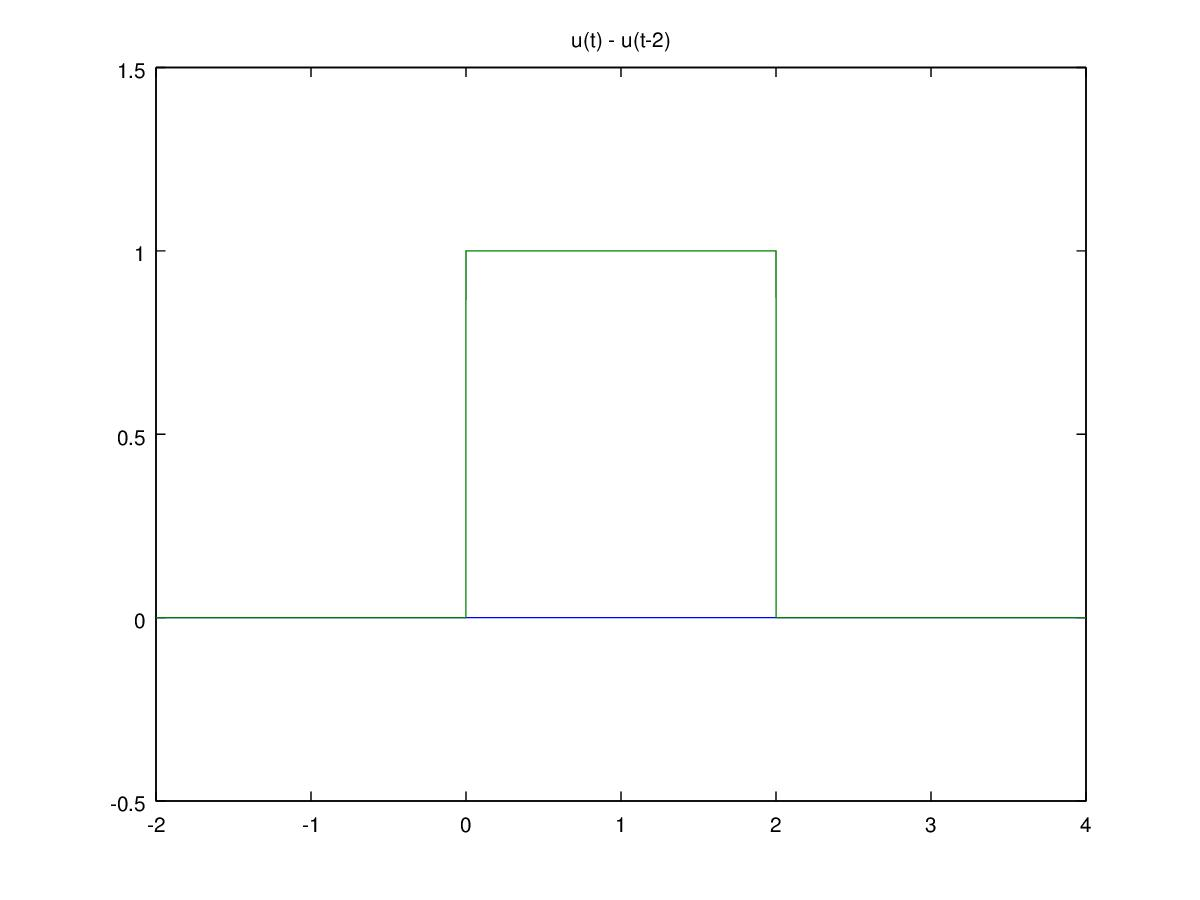
\includegraphics[width=3in]{./graphics/compesccont.eps}
    \caption{Pulso de tiempo continuo con $\tau = 2$}
    \label{compescconteps.3}
  \end{figure}

\subsection{El pulso desplazado}

Un pulso unitario de tiempo continuo $p(t)$ de duraci\'{o}n $\tau$
desplazado en el tiempo $t_{0}$ se define como una diferencia de escalones
unitarios desplazados en el tiempo $t_{0}$
\begin{equation}
  p(t-t_{0}) = \frac{1}{\tau} \, \left(u(t-t_{0}) - u(t - t_{0} -
    \tau) \right).
\end{equation}

\subsection{El impulso como l\'{\i}mite del pulso}

Cuando $\tau$ tiende a $0$, el ancho del impulso tiende a $0$, su
altura tiende a $\infty$, y su \'{a}rea se mantiene igual a $1$.

  \begin{figure}
    \centering
    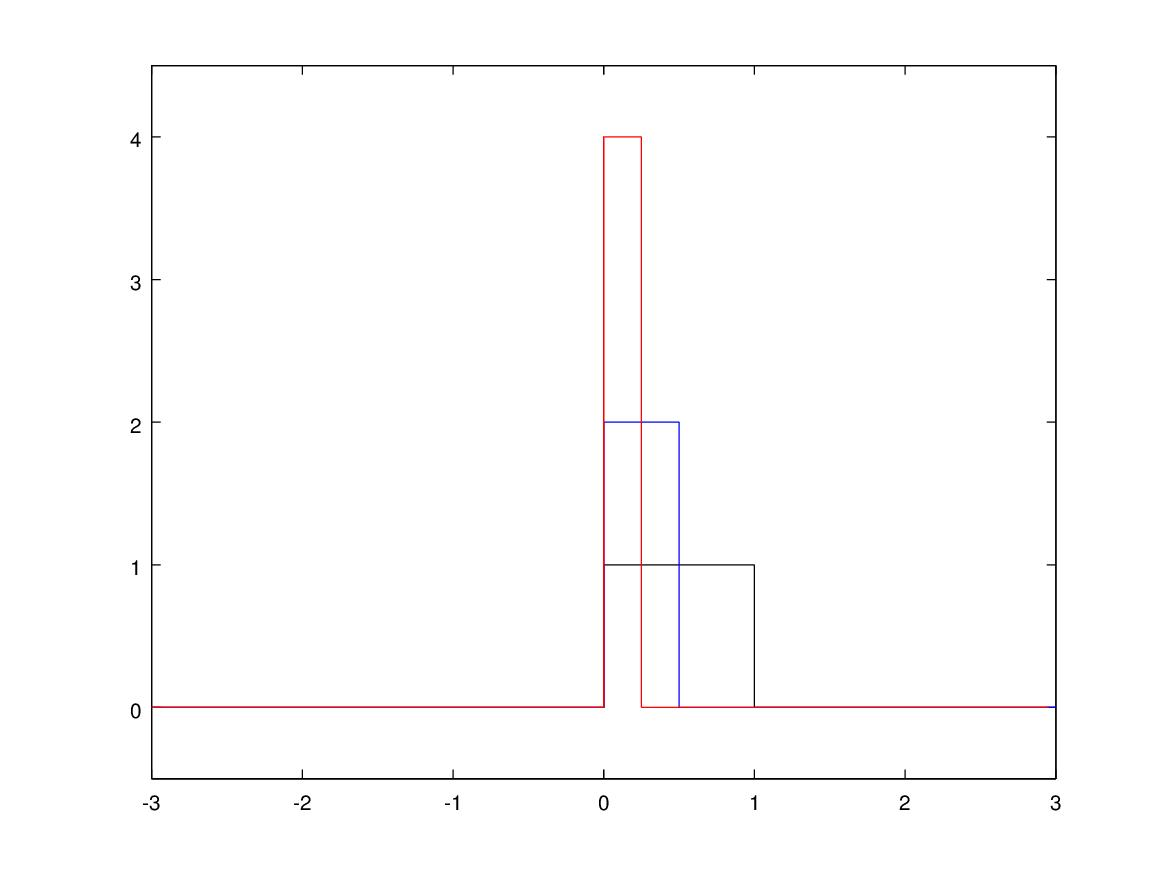
\includegraphics[width=3in]{./graphics/sucimpcont.eps}
    \caption{Impulso como l\'{\i}mite de una sucesi\'{o}n de impulsos}
    \label{sucimpconteps.3}
  \end{figure}

  \begin{figure}
    \centering
    \includegraphics[width=3in]{./graphics/lecture02_tex_gr7.eps}
    \caption{Otra funci\'{o}n de \'{a}rea unitaria (y van dos)}
    \label{lecture02texgr7eps.3}
  \end{figure}

  \begin{figure}
    \centering
    \includegraphics[width=3in]{./graphics/lecture02_tex_gr8.eps}
    \caption{Otra funci\'{o}n de \'{a}rea unitaria (y van tres)}
    \label{lecture02texgr8eps.3}
  \end{figure}

\subsection{La se\~{n}al aproximada por una combinaci\'{o}n lineal de pulsos}

  \begin{figure}
    \centering
    \includegraphics[width=3in]{./graphics/contconv222.eps}
    \caption{Se\~{n}al aproximada por combinaci\'{o}n lineal de pulsos}
    \label{contconv222eps}
  \end{figure}

La se\~{n}al $x(t)$ puede aproximarse como una combinaci\'{o}n lineal
de pulsos desplazados en el tiempo como puede verse en la figura
(\ref{contconv222eps}), o anal\'{\i}ticamente con mediante los
siguientes pasos:
\begin{enumerate}
\item Desplaze los pulsos en el tiempo
\begin{equation}
        \begin{array}{c}
                ...                                             \\ 
                \delta _{\Delta }\left( t+\Delta \right) =
                        \left\{ \begin{array}{l}
                                        \frac{1}{\Delta },      \\ 
                                        0,
                                \end{array}
                                \begin{array}{l}
                                        -\Delta \leq t<0,       \\ 
                                        \left( t<-\Delta \right) \vee \left( 0\leq t\right) ,
                                \end{array}
                        \right.                                 \\ 
                \delta _{\Delta }\left( t\right) =
                        \left\{ \begin{array}{l}
                                        \frac{1}{\Delta },      \\ 
                                        0,
                                \end{array}
                                \begin{array}{l}
                                        0\leq t<\Delta ,        \\ 
                                        \left( t<0\right) \vee \left( \Delta \leq t\right) ,
                                \end{array}
                        \right.                                 \\ 
                \delta _{\Delta }\left( t-\Delta \right) =
                        \left\{ \begin{array}{l}
                                        \frac{1}{\Delta },      \\ 
                                        0,
                                \end{array}
                                \begin{array}{l}
                                        \Delta \leq t<2\Delta , \\ 
                                        \left( t<\Delta \right) \vee \left( 2\Delta \leq t\right) ,
                                \end{array}
                        \right.                                 \\ 
                ...                                             \\ 
                \delta _{\Delta }\left( t-k\Delta \right) =
                        \left\{ \begin{array}{l}
                                        \frac{1}{\Delta },      \\ 
                                        0,
                                \end{array}
                         \begin{array}{l}
                            k\Delta \leq t<\left( k+1\right) \Delta , \\ 
                              \left( t<k\Delta \right) \vee \left( \left( k+1\right) \Delta \leq t\right) .
                         \end{array}
               \right.
        \end{array}
\end{equation}

\item Multiplicando por $x\left( k\Delta \right) \Delta $ al $k-\acute{e}simo$ pulso se obtiene 
\begin{equation}
        \begin{array}{c}
                        ...                                                                    \\ 
                        x\left( -\Delta \right) \delta _{\Delta }\left( t+\Delta \right) \Delta =
                                \left\{ \begin{array}{l}
                                                \frac{x\left( -\Delta \right) }{\Delta }\Delta ,        \\ 
                                                0,
                                        \end{array}
                                        \begin{array}{l}
                                           -\Delta \leq t<0,                                       \\ 
                                          \left( t<-\Delta \right) \vee \left( 0\leq t\right) ,
                                        \end{array}
                                \right.                                                                 \\ 
                        x\left( 0\right) \delta _{\Delta }\left( t\right) \Delta =
                                \left\{ \begin{array}{l}
                                                \frac{x\left( 0\right) }{\Delta }\Delta ,               \\ 
                                                0,
                                        \end{array}
                                        \begin{array}{l}
                                                0\leq t<\Delta ,                                        \\ 
                                                \left( t<0\right) \vee \left( \Delta \leq t\right) ,
                                        \end{array}
                                \right.                                                                 \\ 
                        x\left( \Delta \right) \delta _{\Delta }\left( t-\Delta \right) \Delta =
                                \left\{ \begin{array}{l}
                                                \frac{x\left( \Delta \right) }{\Delta }\Delta ,         \\ 
                                                0,
                                        \end{array}
                                        \begin{array}{l}
                                                \Delta \leq t<2\Delta ,                                 \\ 
                                                \left( t<\Delta \right) \vee \left( 2\Delta \leq t\right) ,
                                        \end{array}
                                \right.                                                                 \\ 
                        ... \\ 
                        x\left( k\Delta \right) \delta _{\Delta }\left( t-k\Delta \right) \Delta =
                                \left\{ \begin{array}{l}
                                                \frac{x\left( k\Delta \right) }{\Delta }\Delta ,        \\ 
                                                0,
                                        \end{array}
                       \begin{array}{l}
                             k\Delta \leq t<\left( k+1\right) \Delta ,               \\ 
                             \left( t<k\Delta \right) \vee \left( \left( k+1\right) \Delta \leq t\right) .
                       \end{array}
                       \right.
        \end{array}
\end{equation}
\item Observe que un valor dado de $t$ (por ejemplo $t_{0})$ s\'{o}lo puede pertenecer a \textbf{un} intervalo 
$k\Delta \leq t<\left( k+1\right) \Delta,$ por lo tanto para $t_{0}$ solo uno de los productos puede ser 
distinto de $0$. Sumando los infinitos productos obtenemos 
\begin{equation}
   x_{\Delta }\left( t\right) =
     \sum_{k=-\infty }^{\infty }x\left( k\Delta \right) \delta
     _{\Delta }\left( t-k\Delta \right) \Delta . \label{funcaspulsessum}
\end{equation}
\end{enumerate}

\subsection{La se\~{n}al como combinaci\'{o}n lineal de impulsos}

Observe que en la ecuaci\'{o}n (\ref{funcaspulsessum}) cuando 
$\Delta$ tiende a cero $x_{\Delta }\left(t\right)$ tiende a 
$x\left(t\right) .$

\begin{equation}
        x\left( t\right) =      
\begin{array}{l}
    Lim \\ 
    \Delta \rightarrow 0
\end{array}
x_{\Delta }\left( t\right) = 
\begin{array}{l}
    Lim \\ 
    \Delta \rightarrow 0
\end{array}
   \sum_{k=-\infty }^{\infty }x\left( k\Delta \right) \delta _{\Delta }\left(t-k\Delta \right) \Delta .
\end{equation}
Adem\'{a}s, cuando $\Delta $ tiende a cero, la sumatoria se convierte en una integral 
\begin{equation}
        x\left( t\right) =\int_{-\infty }^{\infty }x\left( \tau \right) \delta\left( t-\tau \right) d\tau .
\end{equation}
Notemos que por la propiedad del muestreo, debe cumplirse 
\begin{equation}
   x\left( \tau \right) \delta \left( t-\tau \right) = 
     x\left( t\right) \delta \left( t-\tau \right) ,
\end{equation}
y en ese caso 
\begin{equation}
 x\left( t\right) = 
  x\left( t\right) \left( \int_{-\infty }^{\infty }\delta \left( t-\tau \right) d\tau \right),
\end{equation}
con lo que hemos probado que una funci\'{o}n $x(t)$ puede escribirse
como una combinaci\'{o}n lineal de impulsos.

%\subsection{La se\~{n}al multiplicada con un impulso}
%
%Para evaluar la multiplicaci\'{o}n de una se\~{n}al $x(t)$ y un impulso $\delta_{t - t_{0}}$
%consideremos la ecuaci\'{o}n (\ref{funcaspulsessum}). 
%
%\begin{enumerate}
%\item Podemos escribir
%\begin{equation}
%   x_{\Delta }\left( t\right) \, \delta_{\Delta }\left( t-k_{0} \, \Delta \right) = 
%     \left( \sum_{k=-\infty }^{\infty }x\left( k \, \Delta \right) 
%\delta_{\Delta }\left( t-k \, \Delta \right) \Delta \right) \,
%\delta_{\Delta }\left( t-k_{0} \, \Delta \right).
%\end{equation}
%
%\item Esta \'{u}ltima ecuaci\'{o}n es equivalente a 
%\begin{equation}
%   x_{\Delta }\left( t\right) \, \delta_{\Delta }\left( t-k_{0} \, \Delta \right) = 
%   x\left( k_{0} \, \Delta \right) \, 
%  \delta_{\Delta }\left( t-k_{0} \, \Delta \right) \,    
%  \delta_{\Delta }\left( t-k_{0} \, \Delta \right),
%\end{equation}
%pues el pulso en $k_{0} \, \Delta$, al multiplicar a otros pulsos 
%$k \neq k_{0}$, los anula. 
%
%\item Multiplicando ambos lados de la ecuaci\'{o}n por $\Delta$ tenemos
%\begin{equation}
%   x_{\Delta }\left( t\right) \, \delta_{\Delta }\left( t-k_{0} \,
%     \Delta \right) \, \Delta = 
%   x\left( k_{0} \, \Delta \right) \delta_{\Delta }\left( t-k_{0} \,
%     \Delta \right) \, \Delta \, \delta_{\Delta }\left( t-k_{0} \,
%     \Delta \right) \, \Delta,
%\end{equation}
%
%\item Finalmente, tomado el l\'{\i}mite de $\Delta$ tendiendo a $0$ obtenemos
%\begin{equation}
%  \begin{array}{c}
%     Lim \\
%     \Delta \rightarrow 0,
%  \end{array}
%   x_{\Delta }\left( t\right) \, \delta_{\Delta }\left( t-k_{0} \,
%     \Delta \right) \, \Delta = x(t) \, \delta(t - t_{0}),
%\end{equation}
%y
%\begin{equation}
%  \begin{array}{c}
%     Lim \\
%     \Delta \rightarrow 0,
%  \end{array}
%   x\left( k_{0} \, \Delta \right) \delta_{\Delta }\left( t-k_{0} \,
%     \Delta \right) \, \Delta \, \delta_{\Delta }\left( t-k_{0} \,
%     \Delta \right) \, \Delta = x(t_{0}) \, \delta(t - t_{0}).
%\end{equation}
%
%\end{enumerate}
%
%Por lo tanto, $x(t) \, \delta(t - t_{0}) = x(t_{0}) \, \delta(t - t_{0})$.



\subsection{Desplazamiento en el tiempo}

\begin{enumerate}
\item Supongamos una se\~{n}al $x(t)$. Podemos desplazarla en el tiempo
haciendo $y(t) = x(t - t_{0})$.

\item Por ejemplo, si $x_{1}(t) = cos(2 \, \pi \, \frac{2}{10} \, t)$,
  podemos obtener su versi\'{o}n desplazada cuatro unidades de tiempo como
  $y_{1}(t) = x_{1}(t - 4) =  cos(2 \, \pi \, \frac{2}{10} \, (t - 4))$.
\end{enumerate}


\subsection{Escalado temporal}

\begin{enumerate}
\item El escalado temporal es reemplazar la variable independendiente $t$
por otra variable a la que llamaremos $v$. La relaci\'{o}n de estas
variables est\'{a} dada por una escala que simbolizaremos con la letra
$a$. Por ejemplo, $t = a \, v$.

\item Considermos la se\~{n}al $x(t) = sen(2 \, \pi \, t)$. Podemos
  realizar el escalado temporal $t = 2  \, v$, para obtener $y(v) =
  sen(4 \, \pi \, v)$.

\end{enumerate}

\subsection{Tiempo inverso}

Un caso especial de escalado temporal es cuando la escala es
negativa. Por ejemplo, con $t = - v$, obtenemos el denominado tiempo inverso.

\subsection{Tren de impulsos}

\begin{enumerate}
\item Supongamos una serie de impulsos desplazados en el tiempo $\delta(t)$,
$\delta(t - T)$, $\delta(t - 2 \, T)$, $\delta(t - 3 \, T)$ y en
general $\delta(t - k \, T)$, para $k$ entero. 

\item El par de impulsos sucesivos $\delta(t - k \, T)$ y $\delta(t -
  (k+1) \, T)$ esta separado por un intervalo de tiempo $T$.

\item El tren de impulsos es igual a a la sumatoria de todos los
  impulsos $\delta(t - k \, T)$, para $k$ entero
\begin{equation}
\Pi_{T}(t) = \sum_{k=-\infty}^{\infty} \delta(t - k \, T),
\end{equation}
donde los impulsos son no nulos en $t = k \, T$.
\end{enumerate}

\subsection{Muestreo}

El muestreo digital de una señal analógica (de tiempo continuo) nos permite obtener una señal de tiempo discreto.
Si cumplimos ciertas condiciones, que vamos a estudiar durante este curso, 
es posible realizar un proceso inverso que nos permite recuperar la señal de tiempo continuo original.

El muestreo ideal es una función que toma los valores de $x(t)$ en los instantes $t = k \, T$, y $0$ para todo $t \neq k \, T$, 
donde $T$ es el período de muestreo y $k$ es una variable entera. Matemáticamente, podemos representar la operación de muestreo como 
la multiplicación de una señal $x(t)$ con un tren de impulsos de período $T$
\begin{equation}
 y(t) = x(t) \times \Pi_{T}(t) = x(t) \times \left( 
 \sum_{k=-\infty}^{\infty} \delta(t - k \, T)
 \right).
\end{equation}
Entonces
\begin{equation}
	y(t) =  
	\left( 
	\sum_{k=-\infty}^{\infty} x(t) \times \delta(t - k \, T)
	\right) =
    \sum_{k=-\infty}^{\infty} x(k \, T) \times \delta(t - k \, T).
\end{equation}


\section{Operaciones útiles, para tiempo discreto}

% Lathi, página 287

\subsection{Decimación}

Supongamos una señal $x[n]$. La decimación de una señal $x[n]$ es la generación de una nueva señal $y[n]$ mediante la eliminación de ciertas muestras de $x[n]$. 
Para eso multiplicamos $x[n]$ por
\begin{equation}
	y[n] = x[n] \times \left( \sum_{k=-\infty}^{\infty} \delta[n - k \, N]\right),
\end{equation}
Si escribimos
\begin{equation}
	y[n] = \sum_{k=-\infty}^{\infty} x[n] \times \delta[n - k \, N] =
	\sum_{k=-\infty}^{\infty} x[k \, N] \times \delta[n - k \, N].
\end{equation}
es evidente que para $n = q \, N + r$, $q \in N$, $0 < r < N$ debe ser $y[n] = 0$, 

\subsection{Interpolación}

Supongamos una señal $x[n]$. La interpolación de una señal $x[n]$ es la generación de una nueva señal $y[n]$ mediante la introducción de nuevas muestras 
calculadas, por ejemplo, como promedios de dos muestras consecutivas de $x[n]$. Por ejemplo,
\begin{equation}
	y[0] = x[0],
\end{equation}
\begin{equation}
	y[1] = (x[0] + x[1]) / 2,
\end{equation}
\begin{equation}
	y[2] = x[1],
\end{equation}
\begin{equation}
	y[3] = (x[1] + x[2]) / 2,
\end{equation}
y así sucesivamente.

Esta no es la única forma de interpolar. Es sólo un ejemplo de un tema que vamos a ver con más detenimiento cuando veamos transformada de Fourier.

